\documentclass[tikz,border=2pt]{standalone}
\usepackage{amsmath,amssymb}
\usepackage{tikz}

\begin{document}
% Purchasing cost accumulates at the constant rate cD (phones: 170 x 2 = 340 per day); it is
% the same for every EOQ policy, so it drops out of the optimisation unless the unit price
% depends on the batch size (discount: 160 x 2 = 320 per day).
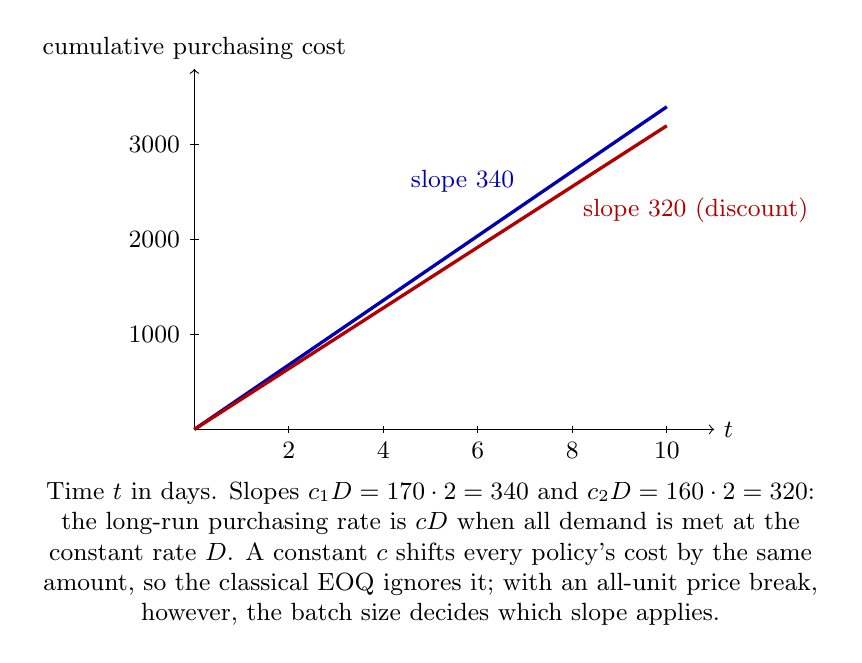
\begin{tikzpicture}[every node/.style={font=\small}, x=0.6cm, y=0.0012cm]
	\draw[->] (0,0) -- (11,0) node[right] {$t$};
	\draw[->] (0,0) -- (0,3800) node[above] {cumulative purchasing cost};
	\foreach \t in {2,4,6,8,10} {\draw (\t,40) -- (\t,-40) node[below] {$\t$};}
	\foreach \c in {1000,2000,3000} {\draw (0.1,\c) -- (-0.1,\c) node[left] {$\c$};}
	\draw[blue!70!black, very thick] (0,0) -- (10,3400) node[pos=0.7, above left] {slope $340$};
	\draw[red!70!black, very thick] (0,0) -- (10,3200) node[pos=0.8, below right] {slope $320$ (discount)};
	\node[anchor=north, align=flush center, text width=10cm] at (5,-450) {Time $t$ in days. Slopes $c_1D=170\cdot2=340$ and $c_2D=160\cdot2=320$: the long-run purchasing rate is $cD$ when all demand is met at the constant rate $D$. A constant $c$ shifts every policy's cost by the same amount, so the classical EOQ ignores it; with an all-unit price break, however, the batch size decides which slope applies.};
\end{tikzpicture}
\end{document}
